\chapter{Time-memory tradeoff}

\footnotesize
\indent \textbf{\textit{Summary.}} Time-memory tradeoff attacks were first conceived on block ciphers by Hellman in 1980. In this approach, Hellman proposed a method for carrying out the precomputation phase of the attack i.e. computing the precomputation tables. We refer to these tables as Hellman tables for block ciphers, in the remainder of the thesis. The proposed idea is based on the birthday paradox, and is thus probabilistic in nature, as we shall see in a moment. 

Later, using this approach as the basis, Shamir and Biryukov proposed a table structure for stream ciphers. This takes into account the amount of keystream available for the attack. We call these tables as Hellman tables for stream ciphers. We start by explaining the original idea of Hellman based on block ciphers. This is done by first presenting a naive approach to building tables for time-memory tradeoff attacks on block ciphers. Then, we point out limitations to the approach and explain how they are improved, consequently leading to the original idea of Hellman. From there, we provide the idea of Shamir and Biryukov, which is used for implementing a time-memory-data tradeoff attack on HiTag2 cipher.

\normalsize
\section{Time-memory tradeoff attack}

\noindent \textit{\textbf{Brute force attack.}} A brute force attack on a block cipher would be to try out all the possible keys which could be used to encrypt certain known (or chosen) or unknown plaintext. The key which decrypts the ciphertext to give the known plaintext or most sensible plaintext (if it is unknown) is then the original key. Though very simple in theory, brute force attacks require a very long time to break ciphers in practice. There is no storage required during this attack, but the time required to break the cipher is very long. Though modern computers have advanced tremendously in their computational speed over the last some years, design of new ciphers have incorporated longer key sizes to protect against brute force attacks, making brute forcing even more impractical.

For example, in order to break a 32 bit key, we would need to carry out $2^{32}$ decryptions on available ciphertext. Using a 2GHz processor (which is quite common for personal use), we can run $2^{31}$ clock cycles in one second (as 1 giga is $2^{30}$). Since one encryption would take a fixed number of clock cycles, say a modest $2^3$ cycles, by simple calculation, we can have a brute force attack on the cipher in $2^4$ seconds, or 16 seconds. As can be seen, this is a dismally weak key size. For a key size of 48 bits, the brute-force would take $2^{20}$ seconds which is 1048576 seconds, or just more than 12 days. In modern ciphers, the key sizes starting from 128 bits in length are considered safe. AES uses a minimum key size of 128 bits, which can be extended to use 256 bits. So, just to give a feeling of the security of a 128 bit cipher, it would take an order of $10^{30}$ years to brute force the key.\\

\noindent \textit{\textbf{Precomputed ciphertext attack.}} Brute-force attacks are just one side of the coin. The other way of breaking a cipher in a known (or chosen) plaintext attack is to precompute ciphertexts corresponding to all the possible keys and to store the (key, ciphertext) pair in a table in memory. During the attack, the attacker just needs to do a table lookup for the available ciphertext to find the corresponding key. Again, the concept is quite straightforward theoretically, but it also faces the same problem as brute-force attacks, but with a different parameter. A table lookup takes constant time (if efficient hash tables are implemented), so practically the attack time is very less. But, the size of precomputed data is tremendous and the attacker would need huge amount of memory to store this data for the attack phase. 

Let us again take the weaker case of a 32 bit key, which is far from use in today's ciphers. For each of $2^{32}$ possible keys, we need to store 32 bits of key and 32 bits of ciphertext (assuming the plaintext is 32 bits, which could very well be more). This amounts to 64 bits or 8 bytes of data for every possible key. $2^{32}$ such entries would require $2^{32} \times$ 8 bytes which is 32 gigabytes. For a random access memory, 32 GB is a high requirement. For higher key sizes, this requirement gets much away from practicality.\\

\noindent \textit{\textbf{In between time and memory.}} The technique of time-memory tradeoff or TMTO is a way between the above two extreme and practically difficult ideas. TMTO solves our problem by using memory in order to reduce the time for attack, bringing the requirements for time and memory within  practical domains. Before we go into more details of the working of time-memory tradeoff attacks on ciphers, we take a simple example of a general application of such tradeoffs. The example has been taken from \cite{stamp2003out}. \\

\noindent \textit{\textbf{Simple example.}} Consider the problem of finding the number of \textbf{1}'s in the binary representation of a non-negative integer $x$ (which takes $4$ bytes). The simplest algorithm to solve this problem would over 32 operations, pick the value of the least significant bit, add it to a variable \textit{sum} and shift $x$ rightwards by one bit. Variable \textit{sum} would then hold the desired result. The pseudo-code for such an algorithm is shown below.

\begin{lstlisting}[frame=tb]
/* ones_count(x) */
sum = 0
for i = 0 to len(x) - 1
    sum = sum + (x >> i) & 1
next i
return sum
\end{lstlisting}

Here, $>>$ denotes the right shift operation and \& denotes bitwise binary \emph{and} operation. The algorithm performs 32 operations (which is based on the length of the integer) and has nearly no memory requirement. The other approach to solve this problem would be to precompute and store the answer for each of the possible $2^{32}$ integers in memory. This way, just one memory lookup is required to find the result for $x$. But in this case, we need to have a memory of the order of $2^{32}$. 

One middle way between both these approaches would be to store the \textit{sum} for all possible 8 bit numbers, rather than doing it for all 32 bit numbers. Then the memory required would be of the order of $2^{8}$. To find the answer for $x$, we break the integer into blocks of 8 bits, and add the stored \textit{sum} for each of the blocks, by looking them up in the table. If $y_1$, $y_2$, $y_3$ and $y_4$ are the four blocks, such that

\begin{center}
$y_4$ = ($x$ $\&$ $0$xFF)\\
$y_3$ = ($(x >> 8)$ $\&$ $0$xFF)\\ 
$y_2$ = ($(x >> 16)$ $\&$ $0$xFF)\\ 
$y_1$ = ($(x >> 24)$ $\&$ $0$xFF)\\
\end{center}

and if p is the array which stores the \textit{sum} for all the 8 bit numbers, then the desired \textit{sum} for $x$ is calculated by

\begin{center}
$sum = p[y_1] + p[y_2] + p[y_3] + p[y_4]$\\
\end{center}

Four operations are performed in this case, as four lookups are made to the precomputed array $p$. This is just one way of realizing the time-memory tradeoff. If the algorithm stores 4 bit blocks, with their corresponding \textit{sum}, then the number of operations would be eight. Hence the optimal combination of memory and time can be chosen based on the resources at hand and the application. 

So, it is easy to see the advantage gained from tradeoff schemes as compared to schemes based on extreme requirements for time or memory. 

\section{Background}

In this section, we provide some building blocks which would be used throughout the thesis. We first introduce the idea of \textit{birthday paradox} and then introduce \textit{hashtables}.

\subsection{Birthday paradox}
\label{sec:bday-paradox}

\indent \textit{\textbf{General birthday paradox.}} Birthday paradox (or birthday problem or surprise, as it is also called), refers to the fact that in a room of 23 people, two people have the same date of birth with a probability greater than one-half. While there are 365 different possible birthdays in a year (excluding the leap year), the birthday paradox looks surprising and non-intuitive at the first glance. But, the figure has been derived from probability theory and is proved. 
% IMP: need a reference here %

A generalized definition of the birthday paradox for can be formulated as follows: given $n$ random integers where each could have $m$ different possible values, the probability that two of them would have the same value is given by the following equation \cite{menezes}.

\begin{center}
$P(m,n)$ $\approx$ $1 - e^{-{n^2}/{2m}}$
\end{center}

If we replace $m$ by 365, and $n$ by 23 in the above equation, then it can be checked that $P(365,23)$ $\approx$ $0.507$. In addition, $P(365,n)$ rapidly increases as $n$ increases, and the chances of two people having the same birthday becomes nearly $99 \%$ for $n$ = 57. If $m$ is considered to be very large, such that $m \rightarrow \infty$, then the above equation can be reduced, giving us the following condition for chances of nearly $100 \%$. 

\begin{center}
$n$ = $\sqrt{\pi/2 \times m}$
\end{center}

The general birthday paradox is used in cryptography in determining collisions in hash functions. Consider a hash function $H$ with $h$ bits of output. The total number of different outputs the function could produce is $2^{h}$. A collision is said to occur when the hash function produces the same output for two different inputs, i.e. $H(x_1)$ = $H(x_2)$ when $x_1$ $\neq$ $x_2$. Then, according to the birthday paradox, the chances that a collision would occur are close to $100 \%$ after the hash function has produced outputs for $2^{h/2}$ random inputs (if we have $m = 2^h$ and we ignore the factor of $\pi/2$).\\

\indent \textit{\textbf{Variant of the birthday paradox.}} A variant of the birthday paradox (\cite{GeneralizedAttack}) is especially more interesting to us, since it is directly used in TMTO attacks. If we consider two groups of people now instead of just one, then just 17 people are required to be present in each group, so that two people, one from each group, share the same birthday.  

We can generalize the above situation in the following way. We have two groups of random elements each having different number elements, say $n_1$ and $n_2$. The elements are non-negative integers, with both the groups having the same range $m$ for all the integers. According to \cite{menezes}, the probability of at least one coincidence in such a case is given by,
\begin{center}
$P(m, n_1, n_2) = 1 -(1 -\frac{n_2}{m})^{n_1}$
\end{center}

For the condition that $m \rightarrow \infty$, the above relation is reduced to,
\begin{center}
$P(m, n_1, n_2)$ $\approx$ $1 - e^{-{n_{1} n_{2}}/{m}}$
\end{center}

For there to be at least one coincidence, the probability must be $1$. Replacing $P(m, n_1, n_2)$ by $1$ and taking the limit $m \rightarrow \infty$, we get the following condition.
\begin{center}
$n_1 \times n_2$ = $\pi/4 \times m$
\end{center}

\begin{align}
\label{eq:bday-paradox2} n_1 \times n_2 \geq m
\end{align}

The last equation above is the birthday paradox we would be using the analysis of most of the TMTO attacks on HiTag2.

% Add the case of handbook statement, with or without replacements?
% also briefly how this paradox would be applied to the TMTO?

% -------------
% what the simple birthday paradox is %

% generalize it in terms of n %

% introduce birthday attack, define scenario (then take hash as example) %

% what is the variant of birthday paradox %

% meet in the middle attack on DES by diffie hellman %
% a TMTO attack would always use variant of birthday attack %

% Question - How can the variant of the birthday problem be derived from the birthday problem?
% Question - Probability of one-half on 23, or is it one? root(pi * m / 2)
% Question - Is meet in the middle attack a TMTO attack? (I think NO!)
% --------------

\subsection{Hash tables}
\label{sec:hash-tables}


Hash tables are used during the precomputation phase as a data structure to store the (prefix, state) pairs in memory. The advantage that hash tables offer is in terms of the search time. The search time provided by hash tables in the best case and the average case is close to $O(1)$, while the worst case search time is $O(n)$ occurring with very less probability. A very important role is played by the hash function chosen for the table. 

The basic data structure for hash tables consists of a pair of data elements, one for holding the \emph{value} to be stored, and the other which acts as a unique identifier for that value, called the \emph{key}. The hast table is basically an array of such (key, value) pairs. Typically in a normal array, pairs would be stored starting from the initial index of the array, with the index increasing with every pair. In a hash table, the pairs are not stored consecutively, but in an order which would make searching them more efficient at a later stage. The index at which a particular pair is stored depends on the key and the hash function. A hash of the key is calculated, and if required, reduced to the domain of the indices. The pair is stored at that index. 

While retrieving a value, the corresponding key is provided and hash of the key is calculated, giving the index of the pair. The index is used to retrieve the value from the array, which is a constant time operation. So, in the ideal scenario, a hash table can provide a constant time search algorithm. But due to the problem of collision, the search time increases by a certain factor. Collision occurs, if the same hash value (thus the same index) is computed for two different keys. In such a case, two different (key, value) pairs would contend to be stored at the same index, thus colliding.

Several proposals have been suggested to avoid the problem of collision. The most popular among them are linear probing and separate chaining. We discuss separate chaining here, since we have implemented this scheme for the two attacks in this section. The basic idea behind separate chaining is that if there is a collision at a particular index, a separate chain holding all the pairs for that index be created. In addition, a reference to the chain must be stored at that index in the array. During retrieval, the index is computed and the reference to the chain is taken from that index. At the reference location, the required value is retrieved by searching through the entire chain. 

The implementation of the hash table is done by Christopher Clark and has been taken from the web source \cite{hash-table-impl}, with due acknowledgment. 

% Also, $M$ is used in defining the hash function for the hashtable. A very simple hash function is used, which uses maps the key to the space $M$ by taking the modulo $M$ of the key.


\section{Babbage-Golic attack}
\label{sec:bg-attack}
Time-memory tradeoff attacks on stream ciphers are relatively new than those on block ciphers. The first TMTO attack which was conceptualized on the block cipher DES, was published by Hellman in 1980 \cite{hellman1980ctm}. In contrast, the first and the simplest TMTO attack on stream ciphers was published by Babbage \cite{babbage} and Golic \cite{golic}, independent of each other in 1995 and 1997 respectively. We would call this attack on stream ciphers as the BG attack. We explain the original BG attack and a variant of it in the sections \ref{sec:bg-r} and \ref{sec:bg-nr}.

\subsection{Attack with random precomputation}
\label{sec:bg-r}

As discussed in section \ref{sec:psrg}, PRSG generates a long keystream using a short secret key, to which the bits of the plaintext are \emph{xor}'ed giving the ciphertext bits. In this way, a stream cipher is produced. A simple model of the PRSG taken from \cite{babbage} is shown in figure \ref{fig:psrg-model}. The initial state of the PRSG is $S_0$, which is derived using the secret key and other initialization parameters. The consequent states are indicated by $S_i$. The right arrow represents the update function while the downward arrow represents the output function. We assume that the PRSG incorporates an LFSR having the maximal period of $2^{n} - 1$.

\begin{figure}[h]
	\centering
	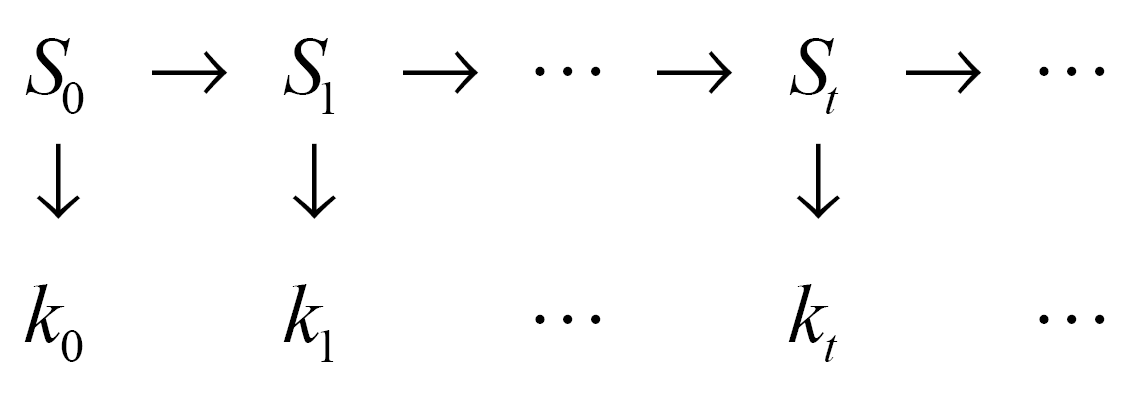
\includegraphics[width=3in]{./figures/prsgmodel.png}
	\caption{Model of pseudo-random sequence generator (PRSG)}	
	\label{fig:psrg-model}
\end{figure}

The keystream bits are represented by $k_0$, $k_1$ $\ldots$, $k_{m-1}$. The goal of the attacker is to find at least one internal state which occurs while the keystream is generated. The attacker could then move the PRSG forward to generate more keystream, in case the keystream is limited. The found internal state could also be used to run the PRSG backwards and find the initial state. From the initial state, finding the key is not a difficult task if the cipher algorithm and initialization parameters are known.\\

\indent \textit{\textbf{Prefix of the output sequence of states.}} If the current state of the PRSG is $S_r$, then an infinite output sequence can be generated by clocking the PRSG from that state. The first $p$ bits of this output sequence is called the prefix of state $S_r$ and would be represented by the bits $k_r$, $k_{r+1}$ $\ldots$, $k_{r+p-1}$. Each of the $2^{n} - 1$ possible states of the PRSG would generate such an output sequence. The prefix of these sequences are usually unique to that particular state if $p$ is greater than or equal to $n$ \cite{biryukov2000rtc}. If the size of the prefix is less than $n$, then there would be many states which could possibly generate this prefix. For example, if the size of the state is 48 bits and we consider prefixes of size 32 bits, then the total number of states which generate this prefix is about $2^{48} \times 2^{-32}$ = $2^{16}$. If the size of the prefixes is increased to 48 bits which is also the size of the state, then there is usually just one state generating the prefix. By increasing the prefix length, the probability that the prefix is unique to the state increases. An advantage of this property is taken in the BG attack.\\

\indent \textit{\textbf{The attack.}} We have two phases in the attack just as in any TMTO attack: the precomputation phase and the attack phase. During precomputation, the attacker randomly selects $n_1$ states out of the $2^n - 1$ possible PRSG states. For each of these states, the prefix of size $p$ = $n$ is computed, and the (prefix, state) pair stored in memory. The data structure that is used for storing the pairs is a hash table, introduced in section \ref{sec:hash-tables}.

During the attack phase, the attacker is assumed to know some part of the initial keystream. In practice, the attacker would know the ciphertext bits. And assuming that the attacker knows the plaintext bits by some means (a known plantext attack), the keystream is simply calculated in the following manner, $k_i$ = $p_i \oplus c_i$, as also mentioned in chapter \ref{chapter:intro}. The attacker then selects overlapping subsequences of size $p$ from the keystream. The first subsequence would be $k_0$, $k_1$ $\ldots$, $k_{p-1}$, the second subsequence would be $k_1$, $k_2$ $\ldots$, $k_{p}$ and so on. The attacker then matches each of these subsequences with the prefix's stored in the hash table. If there is a match, the current state is retrieved from the matched (prefix, state) pair.\\

\indent \textit{\textbf{Parameters in the attack.}} Before we proceed to an analysis of the above attack, we introduce the notation of important parameters used to describe the BG attack. These parameters would help us in understanding where an ideal line be drawn between memory and time consumption during the precomputation and attack phases, so that the attack is feasible say for example on a personal computer. These parameters are introduced below. 

\begin{enumerate}
\item \emph{M} represents the order of memory size required for precomputation.
\item \emph{P} represents the order of time required for precomputation.
\item \emph{T} represents the order of time required for the attack phase.
\item \emph{D} represents the order of data available during the attack phase (applies only to stream ciphers).
\end{enumerate}

\textit{\textbf{Tradeoff equation.}} Let us assume that we select $n_1$ states during the precomputation phase and during the attack phase the PRSG traverses through $n_2$ states before the first match is observed. $M$ is equal to $n_1$, since the size of the hashtable would depend on the number of states stored in it. Similarly, the time to prepare the hashtable is proportional to $n_1$, hence the order of this time, or $P$, is $n_1$. As a result, $M$ = $P$ = $n_1$.

The time taken for the attack or $T$ is the same as $n_2$. The amount of data available or the number of subsequences of length $n$ derived using the available keystream, must be the same as $T$. Hence, $D$ = $n_2$. The keystream should have a length of at least $(D + n - 1)$ bits in order to provide the required amount of data. In such a case, the attacker would have exactly $n_2$ subsequences of length $n$ each to cover the attack time of an order $n_2$.

This is a clear setting for applying the birthday paradox. In a set of $2^n$ states, $n_1$ are selected in precomputation and $n_2$ are selected during the attack. According to the variant of the birthday paradox, explained in section \ref{sec:bday-paradox}, we then have the following condition:

\begin{center}
\large{$n_1 \times n_2$ $\geq$ $2^n$}\\
\large{$M \times T$ $\geq$ $2^n$}\\
\end{center}

This is the condition that we required for a successful attack. Though this is probabilistic, we know that if the parameters of $M$ and $T$ are wisely chosen, the probability of a match becomes very high.

\subsection{Attack with non-random precomputation}
\label{sec:bg-nr}

The precomputation in BG attack is done by randomly generating states of $n$ bits, and then computing their prefix. The other way of performing the precomputation is by selecting states through a deterministic algorithm. Consider that the internal state in a stream cipher runs through all $2^n - 1$ possible states, represented by a huge cycle of states as shown in figure \ref{}. If we select states at a fixed distance $d$ from each other during precomputation, we can be sure that there would be a match if the attack phase has a time order of $d$ \cite{erik-discussions}. This is the main idea behind non-random precomputation and is explained in detail in the further paragraphs. The HiTag2 cipher is well suited for this attack, since it's internal state runs through the longest possible cycle of size $2^n - 1$. The attack phase for this attack remains the same as in case of randomly selected precomputation states.\\

\indent \textit{\textbf{Non-random precomputation phase.}} During the precomputation phase, the selection of states is not done at random. Only an initial state is selected at random for precomputation ($S_{initial}$), while the remaining states are derived using this state. The prefix for $S_{initial}$ is first computed and the (prefix, state) pair stored in the hash table. The next state is derived using a \emph{state transition function} (explained in detail later), which returns the state $d$ states ahead of the current state. The next state then is represented by $S_{initial+d}$. Similarly, the prefix for $S_{initial+d}$ is computed and the (prefix, state) pair stored in the hash table. The process is repeated, and consequently we have a set of states (and the corresponding prefix) in memory. These would be $S_{initial}$, $S_{initial+d}$, $S_{initial+2d}$ and so on. Until the complete circle of states is covered (after which the same states are repeated) we have unique (prefix, state) pairs. At the end of the precomputation phase, we would have a total of $2^n/d$ states in the hash table. The precomputation phase would take memory space of an order of $2^n/d$. It can be clearly seen that $M$ and $P$ would be the same in this case as well, and we have the relation $M$ = $P$ = $n_1$ = $2^n/d$.\\

\indent \textit{\textbf{Attack phase.}} Let us assume that the initial state generating the available keystream is $S_{unknown}$ (as this state is unknown to the attacker). The attacker selects subsequences from the keystream and matches them with the prefixes stored in the memory. If the attacker gets $d$ subsequences from the keystream (which represent $d$ unknown states), a prefix in the memory is bound to get matched with a keystream subsequence. Hence, in the worst case, a traversal through $d$ states would be required during the attack phase, taking $d$ order of operations before a match in the memory. $T$ in this case would be $T$ = $n_2$ = $d$, while $D$ becomes $D$ = $(d + n - 1)$.\\

\indent \textit{\textbf{Tradeoff equation.}} It can be clearly seen that the following relation holds,

\begin{align}
\label{eq:tmto-non-random} M \times T = 2^n
\end{align}

Using this equation, the tradeoff in memory and time can be achieved. It is interesting to compare this equation with the equation for BG attack with random states during precomputation. The latter was based on the birthday paradox, and hence the probability of finding a match is always close to \textbf{1}, but not exactly \textbf{1}. The greater the value of $M \times T$ is as compared to $2^n$, more is this probability closer to \textbf{1}.

In case non-random states are chosen during precomputation, the probability of a match is exactly \textbf{1}, provided the above tradeoff equation holds. This ofcourse assumes that $n$ bits of prefix uniquely identify the state generating it. But this is not the case always, as we shall see from our implementation results. In order to be sure that the prefix uniquely identifies a state, a greater length of prefix should be chosen.\\

\indent \textit{\textbf{Matrix representation of state transition function.}} As mentioned above, the \emph{state transition function} is used in the precomputation phase for deriving a non-adjacent state from the current state. If we use the update function in order compute the state $d$ distance ahead, the function would be called $d$ times and thus take a total computation time of an order $d$. If this has to be repeated in order to cover the entire cycle of states, the computation time required would be of the order of $2^n$. Ofcourse, this is not feasible, otherwise we would very well launch a brute force attack on the internal state. A function is required which derives the $d$'th state in constant time, thus reducing the precomputation time order to $2^{n}/d$. We call such a function the state transition function, and its design is discussed here. 

An update function is used in deriving the adjacent state, which can be represented by a binary matrix $U$ \cite{trappe2005icc}. This matrix on multiplication with the matrix representing the current state gives the adjacent state matrix. If the current state of the LFSR is $S_{current}$, then the next state $S_{next}$ can be computed by the matrix multiplication shown below.

\begin{center}
\large{$U . S_{current}$ = $S_{next}$}\\
\end{center}

This is represented in the matrix notation as follows.

\begin{center}
\large{
$U.$
$\begin{bmatrix}
s_{n} \\
s_{n-1} \\
\vdots \\
s_{1} \\
s_{0}
\end{bmatrix}$ = 
$\begin{bmatrix}
s_{new} \\
s_{n} \\
\vdots \\
s_{2} \\
s_{1}
\end{bmatrix}$}
\end{center}

The topmost row of $U$ would represent the tap sequence by containing \textbf{1} at positions representing the tap bits, and \textbf{0} otherwise. It is so because this row is multiplied with the current state to give the new bit (the leftmost bit) of the LFSR. The remaining rows of $U$ are setup in such a way that the remaining bits of the LFSR are shifted one place rightwards. It must be noted that the indexing in the matrix is the same as that in the LFSR. Thus, the leftmost position in the any row of $U$ is for the \textbf{48}'th bit of the LFSR, and the rightmost position is for the \textbf{1}'st bit. In addition, in the state matrices $S_{current}$ and $S_{next}$, the topmost position is for the \textbf{48}'th bit of the LFSR, and the bottommost position is for the \textbf{1}'st bit. The matrix $U$ for HiTag2 is shown in figure \ref{fig:hitag2-transition-matrix} as an example.

\begin{figure}[h!]
	\centering
	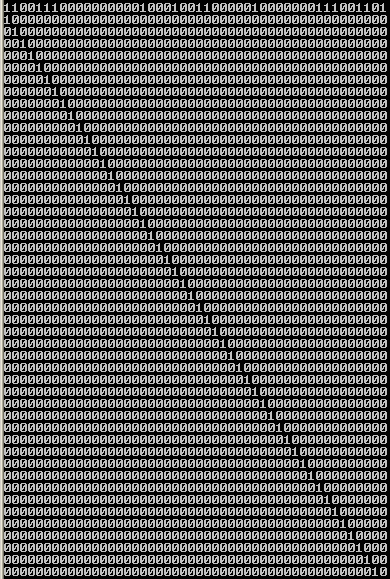
\includegraphics[width=3.5in]{./figures/hitag2-transition-matrix.png}
	\caption{Update function matrix $U$ for HiTag2}	
	\label{fig:hitag2-transition-matrix}
\end{figure}

Matrix multiplication for binary matrices is to perform a bitwise boolean \emph{and} operation (denoted by \&) and then \emph{xor} the resulting bits. In notation, if we have two rows $r_1$ and $r_2$ of size $n$ for multiplication, then we have the following,

\begin{center}
\large{$r_1$ = $r_{11} r_{12} \ldots r_{1n}$}\\
\large{$r_2$ = $r_{21} r_{22} \ldots r_{2n}$}\\
\large{$r_1 \times r_2$ = $(r_{11} \& r_{21}) \oplus (r_{12} \& r_{22}) \oplus \ldots \oplus (r_{1n} \& r_{2n})$}
\end{center}

To compute the state occurring $d$ states after the current state, we perform the above matrix multiplication $d$ times, as follows,

\begin{center}
\large{$S_{current + d}$ = $\underbrace{U . U . U \dots U}_{d} . S_{current}$}, or\\
\large{$S_{current + d}$ = $U^d . S_{current}$}\\
\end{center}

From \cite{erik-discussions}, there is an efficient solution for computing the states. Instead of performing matrix multiplication of $U$ $d$ times, a repeated square of the result can be performed. The square of $U$ is first computed giving $U^2$. This is squared to compute $U^4$, which is again squared to compute $U^8$, and so on. If $\log_2{d}$ is an integer, then the squaring is repeated for $\log_2{d}$ number of times, as shown below.

\begin{center}
\large{$S_{current + d}$ = $\underbrace{(((U^2)^2) \dotsc )^2}_{\log_2{d}} . S_{current}$}\\
\end{center}
\label{eq:state-trans}

As can be seen, computing each state would take $\log_2{d}$ multiplications, and thus the entire precomputation phase would take $d \times \log_2{d}$ matrix multiplications. This is much efficient than the previous complexity of $2^n$. The above equation shall then be used in the precomputation phase of this attack to compute the (prefix, state) pairs.

% It is important to note here that the number of times squaring operation is performed depends only on $M$. 

\subsection{Implementation and results}

Both versions of the BG attack differ in the respective precomputation phase. The attack phase proceeds in the same way for random or non-random precomputation. Ofcourse, the probability of finding the key varies in both the attacks. The module implemented to carry out the complete attack performs the following tasks in sequence,
\begin{enumerate}
\item If the precomputation phase is non-random, a matrix of the state transition function is computed, otherwise it is not. To compute the state transition matrix, the update matrix is first initialized with the tap bits of the LFSR used in HiTag2 and then squared recursively, as discussed in the previous section.
\item The keystream for the attack is made available. A secret key of size $48$ bits is chosen and used in initializing the LFSR along with the serial ID and an initialization vector. Starting with this initial state, the stream cipher is run and keystream of desired length produced and stored in memory. The length of the keystream is defined in terms of the parameter $D$ for the attack.
\item A hashtable of size $M$ is created. If the precomputation phase is non-random, the state transition matrix is used in computing subsequent states which are stored in the hashtable. Else, states are randomly chosen and stored. $P$ defines the number of times a new state is computed (which is not the same as the number of times a new state is stored in hashtable). As we can see, in this case every time a new state is computed, it is stored in the hashtable, hence $P$ and $M$ are the same. We shall see in later attacks that $P$ and $M$ can be different also depending on the algorithm for the precomputation phase. 
\item Lastly, the attack is started. Overlapping subsequences of the prepared keystream are selected and matched with the prefixes in the hashtable. The worst case duration of the attack is the number of subsequences that are available, which is $D$. And thus, in this case we have $T$ = $D$. In some later attacks we shall see that this does not hold. 
\end{enumerate}

% a note about the reversing of keys. little bit of implementation details. (or to mention this in the hitag2 section?)

% a note on random function chosen? %
A random function is required in order to select states for the hashtable in the random precomputation phase. The $rand()$ function provided by $C$ library is not a cryptographically strong function. We implemented a $C$ program to check the period of the output of the $rand()$ function. Following are the observations after running the program.

\begin{enumerate}
\item The output of the $rand()$ function is \textbf{16} bits. This is greatly insufficient for our purpose, since we require random numbers of length \textbf{48} bits. 
\item As expected, the output of the $rand()$ function repeats after around $2^{16}$ calls to the function. The period is unstable, and varies a lot, but remains in the range of $2^{14}$ to $2^{17}$ more or less.
\end{enumerate}

Since, the inbuilt $rand()$ function does not help us in any way, we implemented a random function which uses the $rand()$ function internally. Also we do not require very high level of security from our random function as we generate random states using it, and not keys. Hence, the function solves our purpose. In addition, the period of the function is $2^{27}$ for random numbers of length \textbf{32} bits, which is pretty good for the attacks, as the order of the memory being considered is of the order of $2^{22}$ in the experiments shown below. The program for checking the period of both the $C$ $rand()$ function and our random function is given in appendix.

Three different keys are randomly selected for the attacks. These keys are as follows.

\begin{enumerate}
\item Key $K_1$ = 0x52B49EA34972
\item Key $K_2$ = 0xD4E98D3DA2F2
\item Key $K_3$ = 0x49D2AC801F94
\end{enumerate}

We display the results here for the first two keys $K_1$ and $K_2$ in tables \ref{tab:keystream-attack-results-key1} and \ref{tab:keystream-attack-results-key2} respectively. The detailed output from the attack program corresponding to these results is given in appendix \ref{appendix:tmto-keystream-results}. The values of $M$ and $T$ are varied for each key, for both random and non-random precomputation phase. A very important parameter in the attack is the length of the prefix. We have chosen prefix length of $48$ and $56$ bits for the keys. Low prefix length would lead to higher degree of false alarms, while high prefix length would not matter since \textbf{56} bits of prefix is sufficient in eliminating false alarms. Hence these two values are considered for the experiments. The time taken for the preparation of the hashtable and keystream, and for the attack are all given in seconds. 

\begin{table}[ht!]
\begin{center}
\begin{tabular}{|p{3cm}||c|c|c|c|c|c|c|c|c|c|}
\hline
\multicolumn{11}{|c|}{\textbf{Key $K_1$ = 0x52B49EA34972}} \\ \hline \hline
Precomputation 	& \multicolumn{5}{c|}{Random} & \multicolumn{5}{c|}{Non-random} \\ \hline
Prefix length										&	48 				&	48 				&	48 				&	48 				& 56 				&	48 				&	48				&	48 				&	56 				&	56  			\\ \hline
M																&	$2^{21}$ 	&	$2^{22}$ 	&	$2^{24}$ 	&	$2^{25}$ 	&	$2^{25}$ 	& $2^{21}$ 	&	$2^{21}$ 	&	$2^{21}$ 	&	$2^{21}$ 	& $2^{21}$	\\ \hline
T	  														&	$2^{26}$ 	&	$2^{25}$ 	&	$2^{25}$ 	&	$2^{25}$	&	$2^{25}$ 	& $2^{26}$ 	&	$2^{27}$ 	&	$2^{28}$ 	& $2^{27}$ 	& $2^{28}$	\\ \hline
Time for preparing hashtable		&	16 				&	32 				&	128				&	256				&	279 			& 88 				&	87				& 87				&	89	 			& 89				\\ \hline
Time for preparing keystream		&	6 				&	3 				&	3 				&	3 				&	3 				& 6 				&	12				& 24				&	12				& 24				\\ \hline
Time for attack									&	54 				&	28 				&	29 				&	31 				&	29 				& 56 				&	113				& 223				&	109				& 221				\\ \hline
Number of times key is found		&	0 				&	0 				&	0 				&	2 				&	2 				& 1 				&	1					& 2 				&	1 				& 2					\\ \hline
Number of false alarms					&	0 				&	3 				&	4 				&	7 				&	0 				& 1  				&	2					& 2 				& 0 				& 0					\\ \hline
\end{tabular}
\end{center}
\caption{Results of TMTO keystream attack for key 0x52B49EA34972}
\label{tab:keystream-attack-results-key1}
\end{table}


\begin{table}[ht!]
\begin{center}
\begin{tabular}{|p{3cm}||c|c|c|c|c|c|c|c|c|}
\hline
\multicolumn{10}{|c|}{\textbf{Key $K_2$ = 0xD4E98D3DA2F2}} \\ \hline \hline
Precomputation 	& \multicolumn{4}{c|}{Random} & \multicolumn{5}{c|}{Non-random} \\ \hline
Prefix length										&	48 				&	48 				&	48 				&	56 				&	48 				&	48				&	48 				&	56 				&	56  			\\ \hline
M																&	$2^{22}$ 	&	$2^{23}$ 	&	$2^{22}$ 	&	$2^{22}$ 	&	$2^{22}$ 	&	$2^{21}$ 	&	$2^{22}$ 	&	$2^{22}$ 	& $2^{22}$	\\ \hline
T	  														&	$2^{26}$ 	&	$2^{26}$ 	&	$2^{27}$ 	&	$2^{27}$	&	$2^{25}$ 	&	$2^{26}$ 	&	$2^{26}$ 	& $2^{25}$ 	& $2^{26}$	\\ \hline
Time for preparing hashtable		&	29 				&	58 				&	30 				&	32 				&	178 			&	88				& 178				&	181 			& 181				\\ \hline
Time for preparing keystream		&	6 				&	5 				&	10 				&	11 				&	3 				&	6					& 6					&	3					& 6					\\ \hline
Time for attack									&	70 				&	72 				&	152 			&	148 			&	29 				&	53				& 57 				&	28 				& 55				\\ \hline
Number of times key is found		&	0 				&	2 				&	4 				&	4 				&	1 				&	0					& 1 				&	1 				& 1					\\ \hline
Number of false alarms					&	0 				&	0 				&	1 				&	0 				&	1 				&	0					& 2 				& 0 				& 0					\\ \hline
\end{tabular}
\end{center}
\caption{Results of TMTO keystream attack for key 0xD4E98D3DA2F2}
\label{tab:keystream-attack-results-key2}
\end{table}


The following observations can be made from the above results. 
\begin{enumerate}
\item In column 3 of table \ref{tab:keystream-attack-results-key1}, we can see that $K_1$ is not found even once. On doubling $M$ as shown in the next column, it is seen that $K_1$ is found two times. This indicates that the random function we have in place for generating states for the hashtable does not repeat the states yet. Repeating states would lead to wastage of time and space while creating the hashtable. Hence it is confirmed that the random function and it's usage in the program is good.

\item In column 5 of table \ref{tab:keystream-attack-results-key2}, $K_2$ is found even though the product of $M$ and $T$ is less than $2^{48}$. It is thus clear that equation \ref{eq:tmto-non-random} just indicates the worst case relation between $M$ and $T$. Thus, if the product $M \times T$ $\geq$ $2^{48}$, we can be certain that the key would be found. If $M \times T$ $<$ $2^{48}$, then we cannot be certain. In this particular case, $K_2$ is found. But, another combination of $M$ and $T$ shown in column 6 exemplifies this fact.

\item If the product $M \times T$ = $2^{48}$ for the non-random precomputation, then the correct key is found exactly once. However, if the product $M \times T$ = $2.2^{48}$ (by doubling either of $M$ or $T$), then the correct key is found exactly two times. Also, as can be seen from the appendix, the time between the second match and the first match of the key is precisely $T/2$. For the key $K_1$, the attack output of column 10 is shown below. The point to note here is the percentage of the worst case time for the two matches; they differ by 50\%. 

% NEEDED - see if a figure is needed here.

\begin{lstlisting}[frame=tb]
Match Found! 
Current State: eb444bbc2057  Prefix: d249629ec6a571

Percentage of the worst case time: 19.833907 I: 53241238

Found Initial State: 58c99e374972
Found Key: 52b49ea34972

Match Found! 
Current State: cf258b22b7b5  Prefix: 777609953446b2

Percentage of the worst case time: 69.833907 I: 187458966

Found Initial State: 58c99e374972
Found Key: 52b49ea34972
TIME for attack: 221
\end{lstlisting}

\item It is repeatedly seen that prefix length of 56 bits gives no false alarms, while prefix length of 48 bits does give false alarms. It is clear that 48 bits of prefix are not sufficient to represent a state uniquely. The number of false alarms is not very high though, thus it can also be concluded that for every 48 bit prefix, the number of states giving a same prefix would not be many.
 
\item The attack time for 48 bits prefix is generally more than the time for prefix length 56 bits, under the same $M$ and $T$. This is because false alarms are generated for 48 bit prefixes, and it takes considerable time to find the initial state and then the key from the current state of the LFSR.

\end{enumerate}

\section{Babbage-Golic attack with limited keystream}

In the previous attack, there is an assumption on the length of keystream available to the attacker. The minimum number of operations required to be performed during the attack phase (or $T$) in order to find a match determines the required length of keystream. Considering the use of HiTag2 in car keys, it is certain that long keystream would not be available. Rather several short length keystream (for each transaction between the car and car key) would be available over some span of time. As explained in section \ref{sec:hitag2}, 32 bits of data is exchanged between the car and the car key in the beginning of every run of the protocol. The complete protocol is not known to us, but it is just known that these 32 bits are sent across from the car controller to the key \cite{email-ruptor}. Along with the 32 bits, an IV is also sent. The car key then initializes the HiTag2 cipher using the shared secret key, the IV and its serial ID, and matches the computed output of the cipher to the received 32 bits. These 32 bits of data, known as the \emph{authenticator tag}, perform the function of authenticating the car to the car key. After authentication is successful, subsequent messages if any, are encrypted using the subsequent keystream.

Thus for this particular attack, we assume the availability of authenticator tags to the attacker. Also, we ignore any knowledge of further keystream. Hence the goal is to find the secret key just by using several authenticator tags. The difference between the tags lies in different initial state arising due to a different IV sent by the car. The secret key shared between the car and the car key is the same, and so would be the serial ID of the car key.

\subsection{TMTO tags attack}

The TMTO tags attack consists of the two TMTO phases: precomputation and attack. The precomputation phase involves selecting $M$ different initial states, computing their tags and storing the (tag, initial state) pair in a hashtable. The time for preparing the precomputation phase is of the order of $M$, since the complexity lies in the number of tags chosen for the phase. Hence, we also have $P$ = $M$.

During the attack phase, tags are randomly generated along with their corresponding IV's (to simulate the tags collected by an attacker). These tags are then matched with the tags in the hashtable. For every tag match in the hashtable, the initial state is referred and the key used to initialize the cipher to that state is computed. Since each tag can be generated by approximately $2^n/2^{32}$ states, we cannot be sure that the initial state found is the one we are looking for. Hence, we continue with the matching of further tags until we find that the same key is recovered more than once. Then we can be more sure that it is the correct secret key.\\

\noindent \textit{\textbf{Tradeoff equation.}} Determining the tradeoff equation in the tags attack is discussed here. Getting to the equation is not as straightforward as in the previous attack cases, but the results are strikingly similar.

Let us first consider the probability of finding a match in the hashtable. If the order of the memory required during precomputation is $M$, then we have $M$ different states and corresponding tags. It cannot be guaranteed that all the tags would be different, since a tag would have more than one possible generating states. In the best case, we assume that all the $M$ states generate $M$ different tags. Then, in this case, the probability of getting a tag matched in the hashtable is given by $M/2^{32}$, considering 32 bit tags. We write this probability as $P_1$, such that

\begin{center}
\large{$P_1$ = $M/2^{32}$}
\end{center}

Again, this is the best case probability and the actual probability would be less, since tags would be repeated in the hashtable. Next, we need to determine the probability that a match yields the correct initial state and thus the correct key. This can be determined in the following way: the total number of states is $2^n$ and the total number of tags is $2^{32}$. Then, the probability that the matched tag be representing the correct internal state is $2^{32}/2^n$. This probability is represented by $P_2$ such that

\begin{center}
\large{$P_2$ = $2^{32}/2^n$}
\end{center}

The overall probability of finding the correct state is given by $P$, such that

\begin{center}
\large{$P$ = $P_1 \times P_2$}\\
\large{$P$ = $M/2^{n}$}\\
\end{center}

This is the probability of the correct key being found when we have one tag. Hence, for the probability to be \textbf{1}, the runtime of the attack phase must be of an order of atleast $2^{n}/M$, so that we have $2^{n}/M$ tags. Hence, we can say that

\begin{center}
\large{$T \geq 2^{n}/M$}\\
\large{$M \times T \geq 2^{n}$}
\end{center}

In practice, the product of $M$ and $T$ must be larger than $2^n$, since we considered the best case probability while calculating $P_1$. Practically, $P_1$ would be less than its value in the above equation, which would lead to a lower $P$. With lower $P$, $T$ would have to increased if we want to find the correct state. The equation for $P$ just gives us an approximate value of $M$ and $T$, and it is much probable that the attack is successful for higher values of the two parameters.


\subsection{Implementation and results}

The implementation module for TMTO tags attack executes the complete attack by carrying out the following tasks in sequence. 

\begin{enumerate}

\item Only the non-random precomputation phase for this attack is chosen. Hence the first step is to initialize the update function matrix and state transition matrix.
\item The hashtable is prepared. A fixed 48 bit value is used as the starting state, and equidistant states and their prefixes are stored in the hashtable, with the prefix as the hashkey and state as the hashvalue. The size of the hashtable is $M$, and thus the distance between each state stored is fixed to $2^{48}/M$. Also, the time for preparing the hashtable is $P = M$, since each state computed during precomputation is stored in the hashtable.  
\item The required number of tags for the attack are prepared. It is assumed that the attacker captures 32 bit tags and the IV sent along with it when one run of the authentication protocol takes place between the car and the car key. We emulate this scenario in implementation by generating a random IV and subsequently the 32 bits of keystream (tag) using this IV. The (tag, IV) pair is stored in memory, and used when the attack starts. If the data requirement is of an order $D$, then $D$ such tags and corresponding IV's are prepared. 
\item The attack is started. Each prepared tag is searched in the hashtable. For each match, the initial state from hashtable is reversed using the IV corresponding to the matched tag and the constant serial ID, to give a key. All the keys computed using the matched tags are stored and the number of times each key repeats is noted. 
\end{enumerate}

With this, the attack is complete. Keys $K_1$ and $K_2$ are used in the attack with different values of $M$ and $T$. For each chosen value of $M$ and $T$, the time for preparing the hashtable, time for preparing the tags and time for carrying out the final attack phase is noted. All the time is given in seconds. In addition, we also note the number of matches in the hashtable, and the number of these matches which use the correct key i.e. the number of times correct key is found. The results of the attacks is shown in table \ref{tab:tags-attack-results}.

\begin{table}[h!]
\begin{flushleft}
\small{
\begin{tabular}{|p{2.5cm}||c|c|c||c|c|c|c|}
\hline
Key & \multicolumn{3}{c||}{\textbf{$K_1$}} & \multicolumn{4}{c|}{\textbf{$K_2$}} \\ \hline \hline
M																&	$2^{23}$ 	&	$2^{23}$ 	&	$2^{24}$ 	&	$2^{23}$ 	&	$2^{23}$ 	&	$2^{23}$	&	$2^{24}$ 	\\ \hline
T	  														&	$2^{25}$ 	&	$2^{26}$ 	&	$2^{25}$ 	&	$2^{25}$	&	$2^{26}$ 	&	$2^{27}$	&	$2^{25}$ 	\\ \hline
Time for preparing hashtable		&	332				&	331				&	666				&	332				&	331 			&	320				&	667				\\ \hline
Time for preparing tags					&	199				&	399				&	200				&	199				&	399				&	783				&	199				\\ \hline
Time for attack									&	29 				&	57 				&	29				&	29  			&	56				&	128				& 29				\\ \hline
Number of tags matched 					&	66121			&	132559		&	132141		&	66036			&	132106		&	265457		& 131401		\\
																&$\approx 2^{16}$&	$\approx 2^{17}$&	$\approx 2^{17}$&	$\approx 2^{16}$&	$\approx 2^{17}$&	$\approx 2^{18}$ &	$\approx 2^{17}$	\\ \hline
Number of times key is found		&	0 				&	2 				&	2 				&	1 				&	0 				&	4			& 3		\\ \hline
\end{tabular}}
\end{flushleft}
\caption{Results of TMTO tags attack for $K_1$ and $K_2$}
\label{tab:tags-attack-results}
\end{table}

The following comments are made based on these results. 

\begin{enumerate}
\item Consider the values in column 1 for key $K_1$. The estimated probability of getting a particular tag matched in the hashtable is $P_1$ = $M/2^{32}$ = $2^{23}/2^{32}$ = $1/2^{9}$. Then, if we have $T$ tags, the expected total number of matches is $T \times P_1$ = $2^{25} \times 1/2^{9}$ = $2^{16}$. As discussed, we expect $P_1$ to be less than this value, due to repetition of 32 bit prefixes. But from the experimental results, the number of tags matched is slightly more than $2^{16}$. This is not what was expected, but there is a reason for this.
Since the RNG is based on the C $rand()$ function, which uses a linear congruence geenrator, an output can be repeated within the same period of the generator (without the sequence of outputs repeating). Hence, if in our implementation the same IV repeats resulting in the same tag, then the tag is matched at the same place in the hashtable. This adds to the total number of matches. For all the values of $M$ and $T$ for each key, the observed number of tags matched is slightly higher than the expected number due to this reason.

\item The key is not found even once for the parameters shown in column 2 for key $K_2$. The key is expected to be found atleast two times. Though, on doubling the time $T$ for the attack, the number of matches also double and the correct key is found four times, as expected. 

\item If the time for preparing the hashtable for this case is compared with the same in the case of non-random precomputation with unlimited keystream, then it is seen that the former is less than the latter. This is due to the fact that here we are dealing with 32 bit prefixes, while for unlimited keystream we computed prefixes of length 48 bits. The result is that the hashtable is prepared quickly in this case. 

\item the random number is not repeating. 
\end{enumerate}